\documentclass[11pt]{article}
\usepackage{amsmath,amsbsy,amssymb,verbatim,fullpage,ifthen,graphicx,bm,amsfonts,amsthm,url}
\usepackage{graphicx}
\usepackage{xcolor}
%\usepackage[dvipsnames]{xcolor}
\usepackage{algpseudocode}
\usepackage{breakurl}
\usepackage{url}

\newcommand{\mfile}[1]  {{\small \verbatiminput{./#1}}} % Jeff Fessler, input matlab file
\newcommand{\tmop}[1]{\ensuremath{\operatorname{#1}}}
\newcommand{\R}{\mathbb{R}}
\newcommand{\C}{\mathbb{C}}
\newcommand{\Z}{\mathbb{Z}}
\newcommand{\A}{\mathcal{A}}
\newcommand{\minimize}{\operatorname*{minimize\ }}
\newcommand{\maximize}{\operatorname*{maximize}}
\newcommand{\opdet}[1]{\operatorname{\textbf{det}}\left(#1\right)}
\newcommand{\optr}[1]{\operatorname{\textbf{tr}}\left(#1\right)}
\newcommand{\answer}[2][blue]{\ifdefined\AnswerDefine{\color{#1}\it#2}\fi}
\newcommand{\mtx}[1]{\mathbf{#1}}
\newcommand{\vct}[1]{\mathbf{#1}}
\def \lg       {\langle}
\def \rg       {\rangle}
\def \mA {\mtx{A}}
\def \mB {\mtx{B}}
\def \mI {\mtx{I}}
\def \mJ {\mtx{J}}
\def \mU {\mtx{U}}
\def \mS {\mtx{S}}
\def \mV {\mtx{V}}
\def \mW {\mtx{W}}
\def \mLambda {\mtx{\Lambda}}
\def \mSigma {\mtx{\Sigma}}
\def \mX {\mtx{X}}
\def \mY {\mtx{Y}}
\def \mZ {\mtx{Z}}
\def \zero     {\mathbf{0}}
\def \vzero    {\vct{0}}
\def \vone    {\vct{1}}
\def \vu {\vct{u}}
\def \vv {\vct{v}}
\def \vx {\vct{x}}
\def \vy {\vct{y}}
\def \vz {\vct{z}}
\def \vphi {\vct{\phi}}
\def \vmu {\vct{\mu}}
\def \R {\mathbb{R}}


\usepackage{xspace}
\makeatletter
\DeclareRobustCommand\onedot{\futurelet\@let@token\@onedot}
\def\@onedot{\ifx\@let@token.\else.\null\fi\xspace}

\def\eg{\emph{e.g}\onedot} \def\Eg{\emph{E.g}\onedot}
\def\ie{\emph{i.e}\onedot} \def\Ie{\emph{I.e}\onedot}
\def\cf{\emph{c.f}\onedot} \def\Cf{\emph{C.f}\onedot}
\def\etc{\emph{etc}\onedot} \def\vs{\emph{vs}\onedot}
\def\wrt{w.r.t\onedot} \def\dof{d.o.f\onedot}
\def\etal{\emph{et al}\onedot} \def\st{\emph{s.t}\onedot}
\pagestyle{plain}

\title{{\bf Homework Set 2, CPSC 8420, Fall 2024}} % Change to the appropriate homework number
\author{\Large\underline{Matthew Collins}}
\date{\textbf{\Large\textcolor{red}{Due 10/28/2024, Monday, 11:59PM EST}}} % put your name in the LastName, FirstName format
%\date{\today}

\begin{document}
	\maketitle
	

	\section*{Problem 1}
	For Principle Component Analysis (PCA), from the perspective of maximizing variance (assume the data is already self-centered)
	\begin{itemize}
		\item show that the first column of $\mU$, where $[\mU,\mS]=svd(\mX^T\mX)$ will $\maximize \|\mX \bm{\phi}\|^2_2, \st \ \|\bm{\phi}\|_2=1$. (Note: you need prove why it is optimal than any other reasonable combinations of $\mU_i$, say $\hat{\bm{\phi}}=0.8*\mU(:,1)+0.6*\mU(:,2)$ which also  satisfies $\|\hat{\bm{\phi}}\|_2=1$.) 
		\item show that the solution is not unique, say if $\bm{\phi}$ is the optimal solution, so is $-\bm{\phi}$. 
		\item show that first $r$  columns of $\mU$, where $[\mU,\mS]=svd(\mX^T\mX)$ $\maximize \|\mX \bm{\mW}\|^2_F, \st \ \bm{\mW}^T\bm{\mW}=\mI_r$.
		\item Assume the singular values are all different in $\mS$, then how many possible different $\mW$'s will maximize the objective above?
	\end{itemize} 
	
	\section*{Answer}

\subsection*{Part (a)}
Show that the first column of $\mU$, where $[\mU, \mS] = \text{svd}(\mX^T \mX)$, maximizes $\|\mX \bm{\phi}\|_2^2$ subject to $\|\bm{\phi}\|_2 = 1$.

\textbf{Proof:}

The variance of the data when projected onto a unit vector $\bm{\phi}$ is
	\[
	\|\mX \bm{\phi}\|_2^2 = \bm{\phi}^T \mX^T \mX \bm{\phi} \hspace*{10pt} \text{subject to} \hspace*{10pt}\|\bm{\phi}\|_2 = 1
	\]


$\mX^T \mX$ is a symmetric matrix, decompose it as
   \[
   \mX^T \mX = \mU \mS \mU^T,
   \]
   \hspace*{15pt}where $\mU$ is an orthogonal matrix and $\mS$ is a diagonal matrix containing the singular values
   \[
   \hspace*{10pt}\sigma_1 \geq \sigma_2 \geq \dots \geq \sigma_n \geq 0.
   \]
   

Substituting into the objective function
   \[
   \bm{\phi}^T \mX^T \mX \bm{\phi} = \bm{\phi}^T \mU \mS \mU^T \bm{\phi}.
   \]
   Let $\bm{\psi} = \mU^T \bm{\phi}$. Since $\mU$ is orthogonal, $\|\bm{\psi}\|_2 = \|\bm{\phi}\|_2 = 1$. Thus, the expression becomes
   \[
   \bm{\phi}^T \mU \mS \mU^T \bm{\phi} = \bm{\psi}^T \mS \bm{\psi}.
   \]

The quantity $\bm{\psi}^T \mS \bm{\psi}$ is maximized when $\bm{\psi}$ aligns with the eigenvector corresponding to the largest singular value $\sigma_1$. Therefore, the maximum is achieved when $\bm{\phi} = \mU(:, 1)$.

$\hat{\bm{\phi}} = 0.8 \mU(:, 1) + 0.6 \mU(:, 2)$ satisfies $\|\hat{\bm{\phi}}\|_2 = 1$, the contribution from $\sigma_2$ will reduce the value of $\bm{\phi}^T \mX^T \mX \bm{\phi}$ since $\sigma_1 \geq \sigma_2$. Hence, $\mU(:, 1)$ is the optimal choice.

---

\subsection*{Part (b)}
Show that the solution is not unique if $\bm{\phi}$ is an optimal solution, then $-\bm{\phi}$ is also optimal.

\textbf{Proof:}

Consider the objective function 
	\[
	\|\mX \bm{\phi}\|_2^2 = \bm{\phi}^T \mX^T \mX \bm{\phi}
	\]

Take $-\bm{\phi}$
   \[
   \|\mX (-\bm{\phi})\|_2^2 = (-\bm{\phi})^T \mX^T \mX (-\bm{\phi}) = \bm{\phi}^T \mX^T \mX \bm{\phi}.
   \]

The value of the objective function remains unchanged, which implies that both $\bm{\phi}$ and $-\bm{\phi}$ are optimal solutions.

---

\subsection*{Part (c)}
Show that the first $r$ columns of $\mU$, where $[\mU, \mS] = \text{svd}(\mX^T \mX)$, maximize $\|\mX \bm{\mW}\|_F^2, s.t.$ $\bm{\mW}^T \bm{\mW} = \mI_r$.

\textbf{Proof:}

The objective function can be written as
   \[
   \|\mX \bm{\mW}\|_F^2 = \text{Tr}(\bm{\mW}^T \mX^T \mX \bm{\mW}).
   \]
By SVD $\mX^T \mX = \mU \mS \mU^T$,
   \[
   \text{Tr}(\bm{\mW}^T \mU \mS \mU^T \bm{\mW}).
   \]
Let $\bm{\mV} = \mU^T \bm{\mW}$. Since $\mU$ is orthogonal, $\bm{\mV}^T \bm{\mV} = \mI_r$. The objective becomes
   \[
   \text{Tr}(\bm{\mV}^T \mS \bm{\mV}).
   \]
The trace $\text{Tr}(\bm{\mV}^T \mS \bm{\mV})$ is maximized when $\bm{\mV}$ aligns with the first $r$ columns of $\mU$, corresponding to the largest $r$ singular values $\sigma_1, \dots, \sigma_r$. Therefore, $\bm{\mW} = \mU(:, 1:r)$ is the optimal solution.

---

\subsection*{Part (d)}
Assuming the singular values in $\mS$ are different, how many possible different $\bm{\mW}$'s will maximize the objective?

\textbf{Answer:}

Given that the singular values in \(\mathbf{S}\) are all distinct, the optimization problem of maximizing \(\|\mathbf{X} \mathbf{W}\|_F^2\) under the constraint \(\mathbf{W}^T \mathbf{W} = \mathbf{I}_r\) has solutions that can be expressed as:

\[
\mathbf{W} = \mathbf{U}_r \mathbf{Q},
\]

where \(\mathbf{U}_r\) consists of the first \(r\) columns of \(\mathbf{U}\), and \(\mathbf{Q}\) is any orthogonal \(r \times r\) matrix such that \(\mathbf{Q}^T \mathbf{Q} = \mathbf{I}_r\). The set of all such orthogonal matrices \(\mathbf{Q}\) forms the orthogonal group \(O(r)\).

\newpage

\section*{Problem 2}
	Given matrix $\mX\in\R^{n\times p}$ (assume each column is centered already), where $n$ denotes sample size while $p$ feature size. To conduct PCA, we need find eigenvectors to the  largest eigenvalues of $\mX^T\mX$, where usually the complexity is $\mathcal{O}(p^3)$. Apparently when $n\ll p$, this is not economic when $p$ is large. Please consider conducting PCA based on $\mX\mX^T$ and obtain the eigenvectors for $\mX^T\mX$ accordingly and use experiment to demonstrate the acceleration.

	\section*{Answer}

	To efficiently perform PCA when $n\ll p$, the eigenvectors of $\mX^T\mX$ can be obtained from the eigenvectors of $\mX\mX^T$. This is computationally cheaper when $p$ is large and $n$ is relatively small.
	
	By decomposition of $\mX\mX^T$,
	   \[
	   \mathbf{X}\mathbf{X}^T = \mathbf{U} \mathbf{\Lambda} \mathbf{U}^T,
	   \]
	
	The eigenvectors of $\mX^T\mX$ can be obtained from $\mU$.
		\[
		\mathbf{V} = \mathbf{X}^T \mathbf{U} \mathbf{\Lambda}^{-\frac{1}{2}}
		\]
	
	Python code was created below to expiriment and demonstrate the differences between eigenvalues of $\mX^T\mX$ and $\mX\mX^T$.
	The python code iterates through different sample sizes (n) and different feature sizes (p) and keeps track of the time it takes
	to comput the eigenvalues using both $\mX^T\mX$ and $\mX\mX^T$. From the experiment, we expect that the indirect method using $\mathbf{X} \mathbf{X}^T$ 
	will be significantly faster than the direct method when $n \ll p$. The computational complexity of finding eigenvectors of 
	an $n \times n$ matrix $\mathbf{X} \mathbf{X}^T$ is $\mathcal{O}(n^3)$, which is much more efficient when $n \ll p$.
	As can be seen in Figure~\ref{fig:speedup_graph} and Figure~\ref{fig:speedup_table}, for cases where $n\ll p$, 
	the dramatic speedup of using $\mX\mX^T$ can be seen that appears to be very close to $\mathcal{O}(n^3)$.
	
	\begin{figure}[htbp]
    	\centering
    	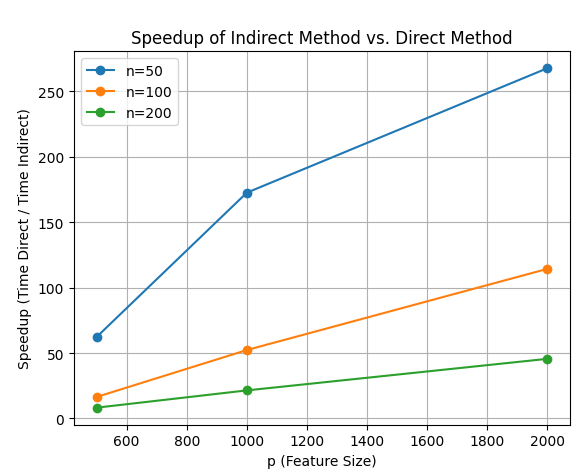
\includegraphics[width=\textwidth]{figures/problem2_graph.png}
    	\caption{Speedup Compared to Feature Size}
		\label{fig:speedup_graph}
	\end{figure}

	\begin{figure}[htbp]
    	\centering
    	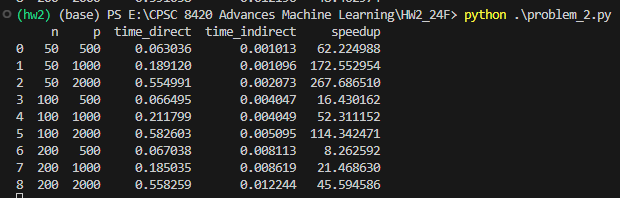
\includegraphics[width=\textwidth]{figures/problem2_table.png}
    	\caption{Speedup Table}
		\label{fig:speedup_table}
	\end{figure}
	
	\subsection*{Python Code}
	
	\begin{verbatim}
	import numpy as np
	import time
	import pandas as pd
	import matplotlib.pyplot as plt

	n_values = [50, 100, 200]
	p_values = [500, 1000, 2000]

	results = []

	for n in n_values:
		for p in p_values:
			np.random.seed(0)
			X = np.random.randn(n, p)

			# Direct Eigenvalue Decomposition of X^T X
			start_time = time.time()
			XtX = np.dot(X.T, X)
			_, V1 = np.linalg.eigh(XtX)
			time_direct = time.time() - start_time

			# Indirect (Efficient Computation) Eigenvalue Decomposition using X X^T
			start_time = time.time()
			XXt = np.dot(X, X.T)
			D, U = np.linalg.eigh(XXt)
			V2 = np.dot(X.T, U) / np.sqrt(D)  # Normalize eigenvectors
			time_indirect = time.time() - start_time

			epsilon = 1e-10
			speedup = time_direct / (time_indirect + epsilon)

			results.append({
				'n': n,
				'p': p,
				'time_direct': time_direct,
				'time_indirect': time_indirect,
				'speedup': speedup
			})

	results_df = pd.DataFrame(results)
	print(results_df)

	for n in n_values:
		subset = results_df[results_df['n'] == n]
		plt.plot(subset['p'], subset['speedup'], marker='o', label=f'n={n}')

	plt.xlabel('p (Feature Size)')
	plt.ylabel('Speedup (Time Direct / Time Indirect)')
	plt.title('Speedup of Indirect Method vs. Direct Method')
	plt.legend()
	plt.grid(True)
	plt.show()

	\end{verbatim}
	\newpage

	
	%\section
	\section*{Problem 3}
	Let $\theta^*\in\R^d$ be the ground truth linear model parameter and $\mX\in\R^{N\times d}$ be the observing matrix and each column of $\mX$ is independent. Assume the linear model is $\vy=\mX\theta^*+\epsilon$ where $\epsilon$ follows $Gaussian(0,\sigma^2\mI)$. Assume $\hat{\theta}=\arg\min\limits_\theta \|\mX\theta-\vy\|^2$.
	\begin{itemize}
		\item Please show that $\mX^T\mX$ is invertible.
		\item Show that $MSE(\theta^*,\hat{\theta}):=E_\epsilon \{\|\theta^*-\hat{\theta}\|^2\}=\sigma^2 trace((\mX^T\mX)^{-1})$
		\item Show that as $N$ increases, $MSE$ decreases. (hint: make use of `Woodbury matrix identity')
	\end{itemize} 

	\section*{Answer}
	\subsection*{Part (a)}
	Show that $\mathbf{X}^T \mathbf{X}$ is invertible.
	
	\textbf{Proof:}

	Each column of $\mathbf{X}$ is independent. The columns of $\mathbf{X}$ form a linearly independent set.
	\[
	\text{rank}(\mathbf{X}) = d, \quad \text{where } d \text{ is the number of columns in } \mathbf{X}.
	\]
	Therefore, if $\mathbf{X}$ has full column rank, then $\mathbf{X}^T \mathbf{X}$ is a $d \times d$ matrix. Since $\mathbf{X}$ has full column rank, $\mathbf{X}^T \mathbf{X}$ is a $d \times d$ matrix, $\text{rank}(\mathbf{X}^T \mathbf{X}) = d$, and $\mathbf{X}^T \mathbf{X}$ is invertible.

	
	\subsection*{Part (b)}
	\textbf{Proof:}
	The estimator $\hat{\theta}$ is given by the least squares solution:
	   \[
	   \hat{\theta} = (\mathbf{X}^T \mathbf{X})^{-1} \mathbf{X}^T \mathbf{y}.
	   \]
	   Substituting $\mathbf{y} = \mathbf{X} \theta^* + \epsilon$, 
	   \[
	   \hat{\theta} = (\mathbf{X}^T \mathbf{X})^{-1} \mathbf{X}^T (\mathbf{X} \theta^* + \epsilon).
	   \]
	Simplifying,
	   \[
	   \hat{\theta} = \theta^* + (\mathbf{X}^T \mathbf{X})^{-1} \mathbf{X}^T \epsilon.
	   \]
	The mean squared error (MSE) is given by:
	   \[
	   \text{MSE}(\theta^*, \hat{\theta}) = \mathbb{E}_\epsilon \left\{ \|\theta^* - \hat{\theta}\|^2 \right\} = \mathbb{E}_\epsilon \left\{ \|(\mathbf{X}^T \mathbf{X})^{-1} \mathbf{X}^T \epsilon\|^2 \right\}.
	   \]
	Since $\epsilon \sim \mathcal{N}(0, \sigma^2 \mathbf{I})$, 
	   \[
	   \mathbb{E}_\epsilon \left\{ \epsilon \epsilon^T \right\} = \sigma^2 \mathbf{I}.
	   \]
	   \[
	   \mathbb{E}_\epsilon \left\{ (\mathbf{X}^T \mathbf{X})^{-1} \mathbf{X}^T \epsilon \epsilon^T \mathbf{X} (\mathbf{X}^T \mathbf{X})^{-1} \right\} = \sigma^2 (\mathbf{X}^T \mathbf{X})^{-1}.
	   \]
	   \[
	   \text{MSE}(\theta^*, \hat{\theta}) = \sigma^2 \text{trace}((\mathbf{X}^T \mathbf{X})^{-1}).
	   \]
	
	---
	
	\subsection*{Part (c)}
	\textbf{Proof:}
	The Woodbury matrix identity states that for matrices $\mathbf{A}$, $\mathbf{U}$, $\mathbf{C}$, and $\mathbf{V}$ of appropriate dimensions:
	   \[
	   (\mathbf{A} + \mathbf{U} \mathbf{C} \mathbf{V})^{-1} = \mathbf{A}^{-1} - \mathbf{A}^{-1} \mathbf{U} (\mathbf{C}^{-1} + \mathbf{V} \mathbf{A}^{-1} \mathbf{U})^{-1} \mathbf{V} \mathbf{A}^{-1}.
	   \]

	where \(\mathbf{A} \in \mathbb{R}^{d \times d}\), \(\mathbf{U} \in \mathbb{R}^{d \times k}\), \(\mathbf{C} \in \mathbb{R}^{k \times k}\), and \(\mathbf{V} \in \mathbb{R}^{k \times d}\).
	Given \(\mathbf{X} \in \mathbb{R}^{N \times d}\), where \( N \) is the number of observations and \( d \) is the number of features.
	Suppose we have an initial sample matrix \(\mathbf{X}_0 \in \mathbb{R}^{N_0 \times d}\) and add a new sample \(\mathbf{x} \in \mathbb{R}^{1 \times d}\).
	The updated observation matrix becomes:
	\[
	\mathbf{X} = \begin{pmatrix}
	\mathbf{X}_0 \\
	\mathbf{x}
	\end{pmatrix} \in \mathbb{R}^{(N_0 + 1) \times d}.
	\]
	\(\mathbf{X}^T \mathbf{X}\) is updated as:
	\[
	\mathbf{X}^T \mathbf{X} = \mathbf{X}_0^T \mathbf{X}_0 + \mathbf{x}^T \mathbf{x}.
	\]

	Let \(\mathbf{A} = \mathbf{X}_0^T \mathbf{X}_0\), \(\mathbf{U} = \mathbf{x}^T\), \(\mathbf{C} = 1\), and \(\mathbf{V} = \mathbf{x}\).
	Applying the Woodbury matrix identity, we get:
	\[
	(\mathbf{X}_0^T \mathbf{X}_0 + \mathbf{x}^T \mathbf{x})^{-1} = \mathbf{A}^{-1} - \mathbf{A}^{-1} \mathbf{U} (1 + \mathbf{V} \mathbf{A}^{-1} \mathbf{U})^{-1} \mathbf{V} \mathbf{A}^{-1}.
	\]
	Simplifying:
	\[
	(\mathbf{X}_0^T \mathbf{X}_0 + \mathbf{x}^T \mathbf{x})^{-1} = (\mathbf{X}_0^T \mathbf{X}_0)^{-1} - \frac{(\mathbf{X}_0^T \mathbf{X}_0)^{-1} \mathbf{x}^T \mathbf{x} (\mathbf{X}_0^T \mathbf{X}_0)^{-1}}{1 + \mathbf{x} (\mathbf{X}_0^T \mathbf{X}_0)^{-1} \mathbf{x}^T}.
	\]

	The term:
	\[
	\frac{(\mathbf{X}_0^T \mathbf{X}_0)^{-1} \mathbf{x}^T \mathbf{x} (\mathbf{X}_0^T \mathbf{X}_0)^{-1}}{1 + \mathbf{x} (\mathbf{X}_0^T \mathbf{X}_0)^{-1} \mathbf{x}^T}
	\]
	is a positive semi-definite matrix. Subtracting this term from \((\mathbf{X}_0^T \mathbf{X}_0)^{-1}\) decreases the overall trace.
	Therefore, as we add more samples (i.e., as \( N \) increases), \(\text{trace}((\mathbf{X}^T \mathbf{X})^{-1})\) decreases, leading to a decrease in MSE.

\begin{thebibliography}{99}

\bibitem{PCAArticle}
Towards Data Science, "Principal Component Analysis (Part 1) — The Different Formulations," \textit{Towards Data Science}, Aug. 30, 2019. [Online]. Available: \burl{https://towardsdatascience.com/principal-component-analysis-part-1-the-different-formulations-6508f63a5553}.

\bibitem{PCAComplexity}
A. Alekhyo, "Computational Complexity of PCA," \textit{Medium}, Jan. 10, 2021. [Online]. Available: \url{https://alekhyo.medium.com/computational-complexity-of-pca-4cb61143b7e5}.

\bibitem{MSEStackExchange}
Stats Stack Exchange, "Is MSE decreasing with increasing number of explanatory variables?" \textit{Stats Stack Exchange}, Dec. 18, 2017. [Online]. Available: \url{https://stats.stackexchange.com/questions/306267/is-mse-decreasing-with-increasing-number-of-explanatory-variables}.

\bibitem{MSEWikipedia}
Wikipedia, "Mean squared error," \textit{Wikipedia, The Free Encyclopedia}, Mar. 1, 2024. [Online]. Available: \url{https://en.wikipedia.org/wiki/Mean_squared_error}.

\bibitem{WoodburyWikipedia}
Wikipedia, "Woodbury matrix identity," \textit{Wikipedia, The Free Encyclopedia}, Mar. 1, 2024. [Online]. Available: \url{https://en.wikipedia.org/wiki/Woodbury_matrix_identity}.



\end{thebibliography}

\end{document}
